\documentclass{article} % For LaTeX2e
\usepackage{nips14submit_e,times}
\usepackage{hyperref}
\usepackage{graphicx}
\usepackage{caption}
\usepackage{url}
%\documentstyle[nips14submit_09,times,art10]{article} % For LaTeX 2.09


\title{Implementing Dimensionality Reduction in Apache Flink using the Lanczos Algorithm}

\author{
Nik Hille \\
\texttt{nik.hille@campus.tu-berlin.de} \\
\And
Fridtjof Sander \\
\texttt{fridtjof.sander@campus.tu-berlin.de}
}

% The \author macro works with any number of authors. There are two commands
% used to separate the names and addresses of multiple authors: \And and \AND.
%
% Using \And between authors leaves it to \LaTeX{} to determine where to break
% the lines. Using \AND forces a linebreak at that point. So, if \LaTeX{}
% puts 3 of 4 authors names on the first line, and the last on the second
% line, try using \AND instead of \And before the third author name.

\newcommand{\fix}{\marginpar{FIX}}
\newcommand{\new}{\marginpar{NEW}}

\nipsfinalcopy % Uncomment for camera-ready version

\captionsetup{justification=centering,width=0.9\textwidth} % Center captions and set width to 90%

\begin{document}

\begin{center}
\textbf{Advanced Information Management III Scalable Data - Analytics and Data Mining}
\end{center}

\vspace{0.8cm}

\maketitle

\vspace{0.8cm}

\vfill

\begin{center}
\today
\end{center}

\pagebreak

\section{Introduction}

\subsection{Dimensionality Reduction and Singular Value Decomposition}

In many applications data can be represented as a matrix that defines a mapping
between two feature spaces. As an example a dataset of ratings of users for
movies may be considered. As depicted in Figure~\ref{fig:exmpl_matrix}, such a
dataset can be modeled as a matrix in which each row represents a user, each
column a movie, and each value a rating that a user has given a movie.

\begin{figure}[h]
\centering
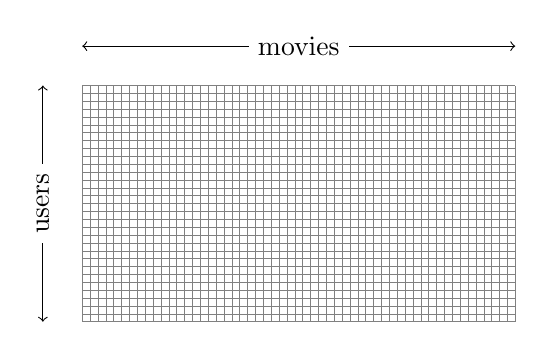
\begin{tikzpicture}
\draw[<->] (0,0.5) -- (0,3.5) node[pos=.5,sloped,fill=white] {users};
\draw[<->] (0.5,4) -- (6,4) node[pos=.5,sloped,fill=white] {movies};
%\draw      (0.5,0.5)  rectangle(6,3.5);
\draw[step=1mm,gray,very thin] (0.4999,0.4999) grid (6,3.5);
\end{tikzpicture}
\caption{Example of a matrix that represents a dataset of ratings from users
for movies}
\label{fig:exmpl_matrix}
\end{figure}

The general goal of such a matrix or vector representation of data is to
exploit well known mathematical functions and properties to process the data,
which is done by many machine learning and data mining algorithms. However, if
at least one feature space is very large, which means in the example that the
number of movies or users is very high, the practical application of this
approach is hindered. The most obvious reason for this roots in the size of the
data, that can get too large as to fit into main memory or as to be processed
efficiently. Beyond that a large number of (possibly dependent) dimensions can
render mathematical functions useless---especially vector distances, on which
important algorithms in machine learning and data mining rely. The latter class
of phenomena is grouped under the term \textsl{curse of dimensionality}.

One approach to tackle the aforementioned problems is called
\textsl{dimensionality reduction} and aims to syntactically and semantically
compress the data's feature spaces by reducing the number of their dimensions.
For instance this would mean in our example to compress the number of movies to
a more abstract concept like genres as depicted in Figure \ref{fig:exmpl_dr}
(in reality, concepts are more fuzzy).

\begin{figure}[h]
\centering
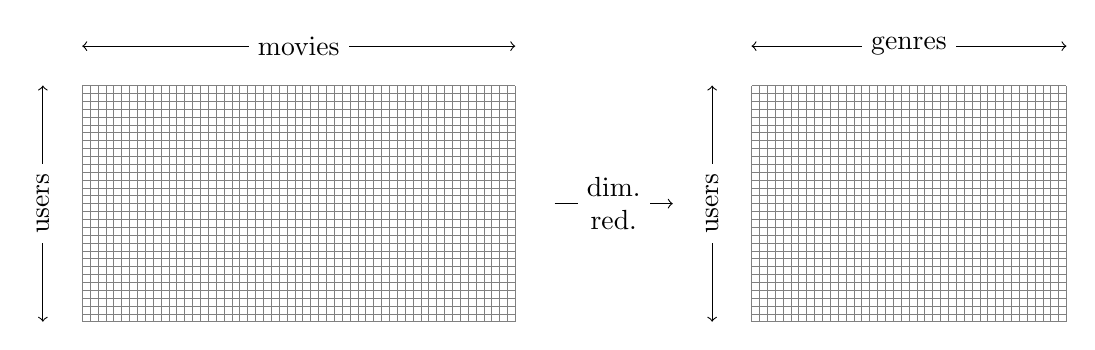
\begin{tikzpicture}
\draw[<->] (0,0.5) -- (0,3.5) node[pos=.5,sloped,fill=white] {users};
\draw[<->] (0.5,4) -- (6,4) node[pos=.5,sloped,fill=white] {movies};
\draw[step=1mm,gray,very thin] (0.4999,0.4999) grid (6,3.5);
\draw[->] (6.5,2) -- (8,2) node[pos=.5,sloped,fill=white, align=center] {dim.
\\ red.};
\draw[<->] (8.5,0.5) -- (8.5,3.5) node[pos=.5,sloped,fill=white] {users};
\draw[<->] (9,4) -- (13,4) node[pos=.5,sloped,fill=white] {genres};
\draw[step=1mm,gray,very thin] (8.9999,0.4999) grid (13,3.5);
\end{tikzpicture}
\caption{Example of dimensionality reduction used to compress the column
feature space from movies to genres}
\label{fig:exmpl_dr}
\end{figure}

This leads to an approximated view of the data, in which a set of movies are
grouped to one or more genres, that are liked or disliked by a set of users.
The approximated data can then be processed more efficiently and sometimes even
more precisely or in a more meaningful way. In \textsl{Latent Semantic
Indexing} for example, a set of documents is indexed by a set of abstract
concepts like topics that are more meaningful to a querying user than a set of
words. The astounding beauty of dimensionality reduction lies in the way it can
be achieved mathematically in an entirely domain agnostic way: With
dimensionality reduction hidden concepts like genres or topics can be
discovered in data that were previously unknown to an investigator. The
abstract concepts like genres or topics are not required to be known in advance
nor is the mapping of concrete feature space dimensions to concepts.

One way of achieving dimensionality reduction is to exploit the
\textsl{Singular Value Decomposition (SVD)} of a matrix. The SVD of a matrix
represents that matrix as a product of three special matrices:

\begin{equation}
	M = U \times \Sigma \times V^T
\end{equation}

$U$ is the basis of the row-feature space and $V$ is the basis of the
column-feature space. So $U$ consists of orthonormal eigenvectors of $M\times
M^T$ and $V$ consists of orthonormal eigenvectors of $M^T\times M$. A
mathematical intuition for this results from building the product of $M$ with
it's transpose and vice versa analog:

\begin{align*}
M \times M^T 	& = (U \times \Sigma \times V^T) \times (V \times \Sigma^T \times
U^T) \\
					& = (U \times \Sigma) \times (\Sigma^T \times U^T) \\
					& = U \times \Sigma^2 \times U^T
\end{align*}

So $U$ and $V$ result from the eigendecompositions of $M\times M^T$ and
$M^T\times M$ respectively. $\Sigma$ is a diagonal matrix that holds the
corresponding square-rooted eigenvalues in descending order. Figure
\ref{fig:svd} gives a more detailed view on the SVD of a matrix $M$.

\begin{figure}[h]
	\centering
	\includegraphics[width=0.8\textwidth]{images/svd_mmds.png}
	\caption{Depiction of the SVD of a matrix $M$ [6]}
	\label{fig:svd}
\end{figure}

The actual reduction of dimensions is then performed by dropping least
significant eigenvalues of $\Sigma$ along with corresponding eigenvectors in
$U$ and $V$ and keeping only the top $k$ one. The resulting matrix in then
called the $\text{rank}_k$ approximation of $M$. This works because the column
vectors of $U$ and $V$ are normalized and thus do not contribute value or
length to a recomposed element. That is entirely done by the eigenvalues of
$\Sigma$. By dropping the smallest values of those, a lowest possible
approximation error is ensured.

\subsection{The Lanczos Algorithm and Eigendecomposition}
\label{ssec:lanczos_algorithm}

In order to compute the SVD of a matrix, the eigendecompositions of $MM^T$ and
$M^T M$ have to be computed:

\begin{align*}
	Eig(MM^T) = (U,\Sigma^2), \;	\;\;	\;\;	\;\;\;	Eig(M^T M) = (V,\Sigma^2)
\end{align*}

This is very expensive if even possible for large matrices, especially when
considered that only the top $k$ eigenpairs are kept. The Lanczos algorithm is
often used as an auxiliary tool, as it provides the possibility to indirectly
compute only the top $k$ eigendecomposition: The Lanczos algorithm takes as
input a symmetric and quadratic matrix $A$ (which is $MM^T$ or $M^T M$ in our
case) and computes as result a matrix $L$ of Lanczos vectors and a symmetric,
tridiagonal auxiliary matrix $T$.

\begin{align*}
	Lanzcos(A) = (L,T) \;\;\;\;\;\;\;\;
L_{m\times k} = \left ( \vec{l_1}, ... \vec{l_i}, ... \vec{l_k} \right )
\;\;\;\;\;\;\;\;
	T_{k\times k} = \begin{pmatrix}  
\alpha_1 & \beta_2  &          & 0 \\
\beta_2  & \alpha_2 & \ddots   & \\
         & \ddots   & \ddots   & \beta_k \\
0        &          & \beta_k  & \alpha_k \\
\end{pmatrix}
\end{align*}

Taking this indirection pays off, because computing the eigendecomposition of
$T$ in the traditional way is very efficient:

\begin{align*}
	Eig(T) = (Q_T,\Lambda_T)
\end{align*}

The eigenvalues of $A$ are then the same as the one of $T$ ($\Lambda_A =
\Lambda_T$) and the eigenvectors of $A$ can be calculated by:

\begin{align*}
	Q_A = L \times Q_T
\end{align*}

As the Lanczos algorithm is the only part in this roadmap that operates on the
large initial data, this is the most crucial part that needs to be
parallelized. The following listing contains a pseudo code variant of the
Lanczos algorithm taken from [5] and [3]:

\begin{flalign*}
\texttt{1}\quad &l_1 \leftarrow \, \text{uniformly distributed vector with norm
1} \\
\texttt{2}\quad &l_0 \leftarrow 0 \\
\texttt{3}\quad &\beta_1 \leftarrow 0 \\
\texttt{4}\quad &\textbf{for} \; j = 1,2,\cdots,k-1\\
\texttt{5}\quad &\qquad w_j \leftarrow A l_j\\
\texttt{6}\quad &\qquad \alpha_j \leftarrow  w_j \cdot l_j \\
\texttt{7}\quad &\qquad w_j \leftarrow w_j - \alpha_j l_j   - \beta_j l_{j-1} \\
\texttt{8}\quad &\qquad \textbf{for}\; i = 1, 2, \cdots,j-2 \\
\texttt{9}\quad &\qquad \qquad w_j \leftarrow w_j - \left(w_j \cdot l_i\right)
l_i \\
\texttt{10}\quad &\qquad \textbf{endfor} \\
\texttt{11}\quad &\qquad \beta_{j+1} \leftarrow \left\| w_j \right\|  \\
\texttt{12}\quad &\qquad l_{j+1} \leftarrow w_j / \beta_{j+1}  \\
\texttt{13}\quad &\textbf{endfor} \\
\texttt{14}\quad &w_k  \leftarrow A v_k \\
\texttt{15}\quad &\alpha_k \leftarrow  w_k \cdot v_k
\end{flalign*}
 
As depicted above the Lanczos algorithm is an \textsl iterive algorithm that
computes in each step $\alpha_j$,~$l_{j+1}$~and~$\beta_{j+1}$ given
$\l_{j-1}$,~$l_{j}$~and~$\beta_{j}$ from the previous step.



\section{Problem Statement}

The goal of our work is to build a program that computes the rank$_k$ approximation of an arbitrary matrix. In the first step, we want to create a program with Apache Flink that runs the Lanczos algorithm in a scalable way for large matrices. After that the intermediate results are passed to an existing solver for eigendecomposition of the Apache Mahout library.

We do not aim to analyze a specific dataset or to draw any domain specific conclusions. We rather want to create a generic tool.

\section{The Lanczos Algorithm}
\label{sec:lanczos}

\section{Approaches}

Before starting the actual implementation process, we first thought about different
ways in which the Lanczos algorithm could be realized in the Apache Flink system. We
identified three different approaches that we could take. One of them would be to
leverage Flink's delta iteration construction, another one would be to make use of
Mahout's implementation of the Lanczos algorithm for the Hadoop framework. The third
possibility we found is to still implement the actual algorithm manually in Flink, but
without using delta iterations to model the algorithm's iterative nature.

% Approach: Delta Iterations
% ==========================

\subsection{Using Flink Delta Iterations}

While planning the implementation part of our project, we consulted both the official
Flink 0.8 documentation [1] as well as the Flink community directly (mainly through
the \#flink IRC channel in the Freenode IRC network) in order to find reasonable
approaches for our intent. The first and most obvious approach both of these sources 
pointed to was to take advantage of Flink's delta iteration capabilities. But what
exactly are delta iterations, how do they compare to standard Flink iterations and why 
would we choose the former over the latter?

% General Description of Flink's Iterations
% -----------------------------------------

Flink provides an iteration operator specifically for the purpose of implementing
iterative algorithms, as these kinds of algorithms occur in many domains of data
analysis and as the general interest in running them on huge data sets is increasing.
The mere existence of this special kind of operator (and the fact that we were explicitly
pointed to it by the Flink community) led us to the conclusion that this must be the
idiomatic way of implementing the Lanczos algorithm in Flink. Two variants of the
iteration operator are provided by Flink: \textbf{Iterate} (we will also call this the
standard iteration) and \textbf{Delta Iterate}. The general idea of both of these operators
is that the programmer defines a step function that will be invoked repeatedly on the
current state of the data until a specified termination condition is reached. [1]

% Iterate Operator
% ----------------

% TODO: Are we allowed to use images from the Flink documentation?
\begin{figure}[h]
	\centering
	\includegraphics[width=0.8\textwidth]{images/iterations_iterate_operator}
	\caption{Graphical representation of the Iterate operator's data flow (source: 
	The Apache Software Foundation [1])}
	\label{fig:iterate_operator}
\end{figure}

Intended to be used for rather simple forms of iteration, the step function (2) of the 
\textbf{Iterate} operator, pictured in figure \ref{fig:iterate_operator}, always takes the 
entire input and computes the next partial solution from that (3). While the first step's input 
is the initial data set specified by the programmer (1), every step that follows consumes the 
partial solution produced by the preceding step. The Iterate operator's final result is simply 
the partial solution produced by the very last step (4). [1]

% Delta Iterate Operator
% ----------------------

\begin{figure}[h]
	\centering
	\includegraphics[width=0.8\textwidth]{images/iterations_delta_iterate_operator}
	\caption{Graphical representation of the Delta Iterate operator's data flow (source: 
	The Apache Software Foundation [1])}
	\label{fig:delta_iterate_operator}
\end{figure}

On the other hand, Flink's \textbf{Delta Iterate} operator, visualized in figure 
\ref{fig:delta_iterate_operator}, is specifically designed for implementing incremental
iterations that only modify small parts of the final result in every iteration step and that 
thus continually evolve the final result rather than fully recomputing it in every step.
Compared to standard iterations, delta iterations bring a performance benefit to the table,
as each of their steps only operates on a small subset of the data. Flink's delta iterations
use a work set and a solution set. While every work set instance only exists for one single
iteration, there is only one instance of the solution set whose state is persisted throughout 
all the iteration steps. The initial values of these two sets (1) are specified by the 
programmer. In every iteration, the step function (2) takes the current work set and the current
state of the solution set as its input and produces a new work set while also (optionally)
updating the contents of the solution set (3). The final result of a delta iteration is
contained in the solution set after the last iteration step has terminated (4). [1]

% Conclusion: Why DELTA iterations for Lanczos?
% ---------------------------------------------

As described in section \ref{sec:lanczos}, every iteration of the Lanczos algorithm only needs
(parts of) the result of the preceding iteration. Also, during every iteration, the final result
is only appended by small parts and none of its existing parts are modified in any way. This
scheme seems to perfectly match the way Flink's delta iterations work, which is why we decided
that delta iterations are more appropriate than standard iterations for implementing the Lanczos
algorithm in Flink.

\subsection{Using Mahout's Lanczos Solver for Hadoop}

% - Idea: Implement interface that Mahout's LanczosSolver uses 
%    --> don't actually implement lanczos in flink

\subsection{Implementing an Iterative, Loop-based Construction}

% --> Flink API/Optimizer doesn't know about iteration
% --> Briefly explain Flink execution strategy/graph (Optimizer)

\section{Implementations}

% Don't draw any conclusions!
% - E.g. stop after saying that the "nested iterations" exception came up!
% - Conclusions belong to the Results/Conclusion sections

This section discusses our attempts at implementing the different approaches
described in section \ref{sec:approaches}. While we won't go over every single
line of our code, we will still give detailed insight into our implementations
in this section.

\subsection{Delta Iterations}

\subsection{Exploiting Mahout's LanczosSolver}


% Loop-Based Implementation
% =========================

\subsection{Loop-Based Implementation}

The loop-based approach discussed in section \ref{ssec:loop_approach} is
actually the one we started implementing first. The basic idea here was to
model the data flow of a single iteration step in Flink and and to implement
the actual iterations using ordinary Java loops. Our first step was to identify
the different modules we would have to develop in order to build a solid
foundation that we could implement the Lanczos algorithm on. The goal here was
not only to make the algorithm's implementation possible, but to provide an API
for ourselves that would make it convenient as well.

% High-Level Project Structure
% ----------------------------

\begin{figure}[h]
	\centering
	\includegraphics[scale=0.5]{images/loop_approach_project_structure}
    \caption{Core project structure of the loop-based implementation}
	\label{fig:loop_project_structure}
\end{figure}

Figure \ref{fig:loop_project_structure} shows the core project structure of our
loop-based implementation. On the top level, it consists of general
\texttt{Config} and \texttt{Utils} classes that contain configuration
parameters and utility functions, respectively. The \texttt{SVD} class acts as
the entry point to the program. Except for some pre- and post-processing, it
basically just invokes the Lanczos algorithm on an input matrix. The
interesting parts of the program are divided into the three sub-packages
\textit{algorithms}, \textit{datatypes} and \textit{operators}. As the
\textit{algorithms} package should be self-explanatory, we will only explain
the general ideas behind the \textit{datatypes} and  \textit{operators}
packages at this point. On that basis, we will then give a lower-level
description of our Lanczos implementation.

% Custom Datatypes
% ----------------

\subsubsection{Custom Datatypes}
\label{ssec:custom_datatypes}

As stated earlier, we aimed for a convenient internal API that would make large
parts of the implementation relatively comfortable for us by hiding
implementation details and by providing powerful abstractions for various kinds
of operations. To achieve this, we developed some custom data types that
provide all the mathematical operations we needed in a convenient way. They can
be found in the \textit{datatypes} package.

% Vector Class
% ------------

The main type of calculation needed in the Lanczos algorithm is vector algebra,
which is why the \texttt{Vector} class is the most verbose and probably one of
the most interesting classes in the project. One step of the Lanczos algorithm
is the multiplication of a matrix by a vector. But as a matrix can be seen as a
list of vectors and as we would have to split the matrix into its row vectors
in order to run this calculation in parallel anyway, we figured we wouldn't
have to implement a separate matrix class.

\begin{lstlisting}[label=lst:vector_usage,captionpos=b,caption=Example use of
the \texttt{Vector} class]
List<Double> v1Elements;
// (Fill the list with 3 vector elements)
Vector v1 = new Vector(v1Elements);
Vector v2 = new Vector.getRandomVector(3, 5); // 3 elements, norm = 5

double v1Norm     = v1.norm();     // L2 norm by default
Vector v1Scaled   = v1.scaleTo(1); // Scale v1 to norm 1
Vector difference = v1.minus(v2);
double dotProduct = v1.dot(v2);
Vector v1Doubled  = v1.times(2);
Vector v2Halved   = v2.divideBy(2);
\end{lstlisting}

Internally, the \texttt{Vector} class simply uses an ordinary Java list of
\texttt{Double} values to store its elements. The class allows new vector
instances to be constructed from a list of elements, from a Java map containing
elements mapped to their indices or by creating a copy of an existing vector.
It also provides static methods for constructing new zero vectors or random
vectors of arbitrary sizes. As for the actual algebra, the \texttt{Vector}
class contains instance methods for calculating a vector's norm, scaling a
vector to any target norm, subtracting one vector from another, building the
dot product of two vectors and multiplying or subtracting a vector by a scalar.
Listing \ref{lst:vector_usage} demonstrates usage of the \texttt{Vector} class
for convenient vector calculations.

% Other Datatypes
% ---------------

Compared to the vector type, the other custom data types are less important and
less interesting. The \texttt{VectorElement} class represents a value that has
an index of some sort, for example an index indicating the value's position in
a vector, but it doesn't implement any algebraic operations on that value.
Because the Lanczos algorithm's final result are two matrices, we wanted to
have a way of returning two matrices from a method, which we solved by wrapping
those two matrices inside the \texttt{LanczosResult} class.

% Custom Flink Operators
% ----------------------

\subsubsection{Custom Flink Operators}
\label{ssec:custom_operators}

Since Flink operates solely on data sets, one has to implement a Flink
program's data flow by defining custom operators and then invoking those
operators on data sets representing the relevant data. This is exactly the
purpose of the modules in our \textit{operators} package. Some of these modules
do calculations on vectors and scalar values, while others only transform
existing data from one form into another.

The operators \texttt{GetVectorNorm}, \texttt{GetVectorNormAsDouble},
\texttt{VectorScalarDivision}, \texttt{DotProduct},
\texttt{VectorScalarMultiplication} and \texttt{VectorScalarSubtraction} are
basically just wrapper classes that allow all the vector operations described
in section \ref{ssec:custom_datatypes} to be invoked on data sets in parallel
(more or less). This is where our custom vector class comes in handy, because
instead of manually working with instances of Java lists or Flink's tuple data
types to perform the necessary calculations, these operators can simply use our
vector API without having to know how the algebraic operations they use are
actually implemented.

\begin{lstlisting}[label=lst:vector_scalar_multiplication,captionpos=b,caption
=Implementation of the custom operator for vector-scalar multiplication]
// (Package definition + imports)

public class VectorScalarMultiplication
    extends RichGroupReduceFunction<Vector, Vector> {
    
  public void reduce(Iterable<Vector> vectors, Collector<Vector> out) {
    double scalar = getRuntimeContext()
                      .<VectorElement>getBroadcastVariable("scalar")
                      .get(0).getValue();
    vectors.forEach(vector -> out.collect(vector.times(scalar)));
  }
}
\end{lstlisting}

For example, our custom operator for vector-scalar multiplication, which
extends Flink's \texttt{RichGroupReduceFunction} and is shown in listing
\ref{lst:vector_scalar_multiplication}, simply uses our vector API's
\texttt{times()} method to calculate and emit the products of a single
broadcasted scalar value with all the vectors contained in the data set the
operator is invoked on. Thanks to the effort initially spent on developing a
custom vector type, we were able to implement most of the Flink operators we
needed very easily.



\section{Results}
\label{sec:results}

In the course of this project, it turned out that at least two of the three
approaches we initially identified are currently unfeasible. The idiomatic
solution using Flink's delta iterations can not be fully implemented, because
nested iterations, which are required to orthogonalize the Lanczos vectors and
thus ensure the correctness of the algorithm's results, are not supported yet
by Flink as of version 0.8.

As described in section \ref{ssec:loop_performance_problem}, the loop-based
approach we implemented is not feasible in practice due to major performance
issues. Our explanation for the observed problems is that the Flink compiler
and/or optimizer is overloaded by the complexity of the execution graph that it
has to generate or optimize, respectively. The problem here is most likely that
Flink can't really recognize the iterative nature of the algorithm. Instead,
before trying to build the execution graph, Flink probably already executes all
loop iterations in oder to determine, which and how many data sets are needed
and how the data flows through the program. At one point during the
investigation of this problem, we looked at a JSON representation of the
program's execution graph. Even though we only used three Lanczos iterations,
the representation of the graph consisted of \textit{several thousand} lines
of JSON. While one single iteration step in our implementation may not seem to
be that complex, we assume that Flink can't handle the complexity of the full
data flow that only unfolds during the attempt of compiling the execution
graph. This explanation seems even more probable considering that the
orthogonalization in every single iteration step is done in a nested loop that
iterates over all previously calculated results again, which adds a lot of
additional complexity to every single iteration.

We had initially discarded the idea of simply using Mahout's implementation of
the Lanczos algorithm by implementing all the interfaces it uses (see section
\ref{ssec:approach_mahout}). But as it stands at the end of our project, this
is the only one of the three identified approaches that could work and be
feasible in current versions of Flink. Unfortunately, we didn't have enough
time left to implement this approach as well and to actually test how well it's
working.


\section{Conclusion}

As of Flink version 0.8, a satisfactory solution for implementing the Lanczos
algorithm doesn't seem to exist yet. The idiomatic approach using delta
iterations and the loop-based approach are either not possible or not feasible.
Using Mahout's implementation of the algorithm would mean taking an
implementation intended to be used specifically with the MapReduce computing
model and squeezing it into the Flink system. While this approach would
probably be possible, we feel that it can't be the 'right' way to do it as it
would undermine many of Flink's individual advantages. Additionally we don't
expect the workaround of materializing all intermediate data to perform
significantly better than Mahout running on Hadoop. This project also
illustrates the current limitations of Apache Flink for implementing iterative
algorithms. In order to develop an idiomatic, satisfactory implementation of
the Lanczos algorithm, one currently has to wait for newer Flink versions that
will support nested iterations.


\subsubsection*{References}

\small{
[1] Alexander, J.A. \& Mozer, M.C. (1995) Template-based algorithms
for connectionist rule extraction. In G. Tesauro, D. S. Touretzky
and T.K. Leen (eds.), {\it Advances in Neural Information Processing
Systems 7}, pp. 609-616. Cambridge, MA: MIT Press.

[2] Bower, J.M. \& Beeman, D. (1995) {\it The Book of GENESIS: Exploring
Realistic Neural Models with the GEneral NEural SImulation System.}
New York: TELOS/Springer-Verlag.

[3] Hasselmo, M.E., Schnell, E. \& Barkai, E. (1995) Dynamics of learning
and recall at excitatory recurrent synapses and cholinergic modulation
in rat hippocampal region CA3. {\it Journal of Neuroscience}
{\bf 15}(7):5249-5262.
}














\end{document}
